\documentclass[twocolumn,showpacs,preprintnumbers,nofootinbib,prd,
superscriptaddress,10pt]{revtex4-1}

\usepackage{amsmath,amssymb}
\usepackage{amsfonts}
\usepackage[normalem]{ulem}
\usepackage{textcomp}
\usepackage{hyperref}
\usepackage{enumitem}
\usepackage{bm}
\usepackage{afterpage}
\usepackage{graphicx}
\usepackage{psfrag}
\usepackage{mathtools}
%\usepackage{tensor}
\usepackage{layouts}
%\usepackage{DejaVuSans}
\usepackage{epstopdf}
\usepackage[usenames,dvipsnames]{xcolor}
\usepackage[utf8]{inputenc}
\usepackage{multirow}
\usepackage{rotating}
\usepackage{tabularx}
\usepackage{ragged2e}
\usepackage{cleveref}
\usepackage{blindtext}
\usepackage{graphicx}
\usepackage{siunitx}
	\sisetup{output-decimal-marker={.}}
\newtheorem{theorem}{Theorem}
\usepackage{float}
	

	%some math symbols
\newcommand{\R}{\mathbb{R}}
\newcommand{\N}{\mathbb{N}}
\DeclareMathOperator{\sign}{sign}
\renewcommand{\d}[1]{\ensuremath{\operatorname{d}\!{#1}}}
%argmin and argmax
\DeclareMathOperator*{\argmax}{arg\,max}
\DeclareMathOperator*{\argmin}{arg\,min}

% comments command
\newcommand{\wdp}[1]{{\textcolor{magenta}{\texttt{WDP: #1}} }}
\newcommand{\amartini}[1]{{\textcolor{blue}{\texttt{AM: #1}} }}
\newcommand{\sschmidt}[1]{{\textcolor{red}{\texttt{SS: #1}} }}

\begin{document}

	%%%%%%%%%%%%%%%%%%%%%%%%%%%%%%%%% ABSTRACT
\begin{abstract}
Burg method of Maximum Entropy Spectral Analysis (MESA) provides a powerful tool to perform spectral estimation of a time-series. The method is a generalization of Jaynes maximum entropy principle and provides the estimate for the spectrum in terms of the coefficients of some autoregressive process AR(p) or order $p$.
A closed form recursive solution provides an estimate of the autoregressive coefficients as well as of the order $p$ of the process.
We provide a ready to use implementation of the algorithm in the form of a python package `memspectrum`. We characterize our code performing a power spectral density analysis on some syntethic generated data (with known power spectral density) and we compare different criteria for stopping the recursion. Furthermore, we compare the performance of our code with the traditional Welch algorithm, using both syntethic data and real gravitational waves data from the LIGO-Virgo collaboration.
We find that, when compared to the Welch's method, the Burg's method provides a power spectral density (PSD) estimation with a systematically lower variance. This is particularly manifest in the case of a little number of datapoints, making Burg method most suitable to work in this regime.
%Several methods are characterized on synthetic noise having a known power spectral density (PSD) via the computation of the percentage error and then compared.  

\end{abstract}
	
	%%%%%%%%%%%%%%%%%%%%%%%%%%%%%%%%% TITLE
	\title{Maximum Entropy Spectral Analysis: a case study}
	\author{Alessandro \surname{Martini}}
		\email{martini.alessandr@gmail.com}
        \affiliation{Dipartimento di Fisica  Università di Pisa, and INFN Sezione di Pisa, Pisa I-56127,Italy}        
	\author{Stefano \surname{Schmidt}}
		\email{s.schmidt@uu.nl}
        \affiliation{add me}      
	\author{Walter \surname{Del Pozzo}}
		\email{walter.delpozzo@unipi.it}
        \affiliation{Dipartimento di Fisica  Università di Pisa, and INFN Sezione di Pisa, Pisa I-56127,Italy}      
  
	
	\maketitle
	\tableofcontents

	%%%%%%%%%%%%%%%%%%%%%%%%%%%%%%%%% BODY  

\section{Introduction}

The study of the properties of  stochastic processes is a crucial task in many fields of physics and mathematical physics [Here we should make some examples...].
A particularly interesting class of stochastic processes are the so-called \textit{wide-sense} stationary processes. These are stochastic processes that display an invariance of their statistical properties, such as their two-point autocovariance function, with respect to time translation. If $x(t)$ is a wide-sense stationary process, it is completely determined by the knowledge of the autocorrelation function 
\begin{equation}
	C(\tau) = \mathbf{E}[x_t \cdot x_{t+\tau}]
\end{equation}
or equivalently by the knowledge of their \emph{power spectral density} (PSD) $S(f)$. Thanks to the Wiener-Khinchin theorem the two are related by a Fourier transform: 
\begin{equation}
	S(f) = \int_{-\infty}^{\infty} \textrm{d}\tau C(\tau) e^{-i 2 \pi f \tau}\,.
\end{equation}
In some literature, the PSD is introduced as  
\begin{equation}\label{eq:psd-f-definition}
	\mathbf{E}[\tilde{x}(f) \cdot \tilde{x}(f^\prime)] = S(f) \delta(f-f^\prime)
\end{equation}
without highlighting its connection with the time structure of the process itself, thus masking some important properties that will explore further in what follows. The latter definition in (\ref{eq:psd-f-definition}) gives, however, i) a straightforward interpretation of the PSD: it measures how much signal ``power" is located in each frequency; ii) an operative way of estimating it for an unknown process.  
%Under such assumption, it can be shown [cite something] that the problem of characterizing the noise properties is greatly simplified and its properties are summarized by a single \textit{autocorrelation function}, which describes how an observation at a given time correlates with another observation a later time. More formally, the properties of a zero mean time series $x_t$ are described by the function:
%\begin{equation}
%	R(\tau) = \mathbf{E}[x_t \cdot x_{t+\tau}]
%\end{equation}
%where the average is computed on different times $t$.
%Thus, a stationary noise time series is completely characterized by the autocorellation function.
%\par
%More often, the study is performed in frequency domain: indeed, for stationary noise the components in frequency $\tilde{x}(f)$ of a stationary time series are conditionally independent from each other. It can be shown that:
%\begin{equation}
%	\mathbf{E}[\tilde{x}(f) \cdot \tilde{x}(f^\prime)] = S(f) \delta(f-f^\prime)
%\end{equation}
%This equation defines the function \textit{power spectral density} (PSD) $S(f)$.
%The PSD has a straightforward interpretation: it measures how much signal ``power" is located in each frequency bin. Furthermore, it is not difficult to show that it is the Fourier transform of the autocorrelation function:
%\begin{equation}
%	S(f) = \int_{-\infty}^{\infty} \textrm{d}\tau R(\tau) e^{-i 2 \pi f \tau}
%\end{equation}
%A power spectral density fully describes a stationary noisy time series and this shows how important is in the study of noise.
%\par
%Thus, in many real application, the knowledge of the PSD is crucial for the understanding of the process and indeed algorithms for PSD computation are a standard part of every software package for computational physics.
A ubiquitous method for such computation is due to Welch \cite{Welch} and it based on the method of periodograms. Basically, the PSD is obtained by slicing the observed realisation $x(t_1),\ldots,x(t_n)$ of the process $x(t)$ into many windowed batches and averaging the squared moduli of their Fourier transforms. The standard approach of periodograms \cite{Lomb,Scargle} consists in taking the Fourier Transform of the sample autocorrelation, written as \begin{equation}
    \rho = \left\{W_0\rho_0,W_{\pm 1}\rho_{\pm 1}, \dots, W_{\pm M}\rho_{\pm M}, 0, 0, \dots \right\}.
\end{equation}
The sequence $W$ is a window function that can be chosen in several different way, each choice presenting advantages and disadvantages for the final estimate of the PSD. \sschmidt{Here we say different things about periodigrams. We should be more clear...}

The choice of a window function is arbitrary and typically is made by trial and error, until a satisfactory compromise between variance and resolution of the estimate of PSD is reached. A high frequency resolution implies high variance and vice-versa. Moreover, the final result depends on the choice of window function, hence begging the question of what the ``real" PSD is. \\  
Another problem with this approach is the requirement for the window to be $0$ outside the interval: we are arbitrarily assuming $\rho_j = 0$ for $j > M$, and modifying the estimate if a non-rectangular window is chosen. Making assumptions on unobserved data and modifying the ones we have at our disposal introduces information about the process that is not really there. Moreover, this method requires a number of arbitrary choices to be made, e.g. the number of time slices, the kind of Window function, the overlap between consecutive slices, etc... All the knobs must be tuned by hand and their choice can dramatically affect the PSD estimation.
\par
An appealing alternative approach, based on the Maximum Entropy principle \cite{Jaynes}, has been put forward by Burg \cite{burg1975maximum}. Being rooted on solid theoretical foundations, we will see that Burg's method, unlike Welch's, does not require any preprocessing of the data and requires very little tuning of the arbitrary parameters, as it provides an iterative closed form expression for the spectrum of a stochastic time series. Furthermore, it embeds the PSD estimation problem into an elegant theoretical framework and makes minimal assumptions on the nature of the data.
Lastly and most importantly, it provides a robust link between spectral density estimation and the field of autoregressive processes. This provide a natural and simple machinery to forecast a time series, thus predicting past observations based on previous ones.

In this paper we discuss the details of the Maximum entropy principle, its application to Power Spectral Density estimation with Burg algorithm and the link between Burg's algorithm and autoregressive process. Furthermore, we present and describe a new code, \texttt{memspectrum}, that provides a robust python implementation of the algorithm.
We provide a thorough assessment of the performance of our code and we validate our results performing a number of tests. We compare our results with those of spectral analysis carried out with the standard Welch method.
\par
Our paper is organized as follows: blablabla...


\section{Theoretical foundations}
The Maximum Entropy principle (MAXENT) is among the most important results in Bayesian probability theory. It provides a way to uniquely assign probabilities to a phenomenon in a way that best represent our state of knowledge, while at the same time it is non committal with unavailable information. Its domain of application turned out to be wider than expected. In fact, thanks to Burg \cite{burg1975maximum}, this method has also been applied to perform high quality computation of power spectral densities of time series.

After a short introduction to Jayne's MAXENT (sec.~\ref{sec:MAXENT}), we will develop in detail Burg's technique of Maximum Entropy Spectral Analysis (MESA) and show that the estimate can be expressed in an analytical closed form (sec.~\ref{sec:MESA}).
Next, we will discuss an interesting link between Burg's method and autoregressive processes (sec.~\ref{sec:autoregr}) and in sec.~\ref{sec:forecasting} we will use such link for straightforwardly forecasting a time series.

\subsection{Maximum Entropy Principle} \label{sec:MAXENT}

Before introducing MAXENT as a variational problem, we will workout some simple examples to contexualise how information's entropy
and `uncertainty' are related. First of all,  it is worth noting that the word `information' will not be used to indicate our knowledge on the system under study: this is what we will call `evidence'. Information will be intended as in communication theory: it specifies the length of the message necessary to provide
a full description of the system under study.

For instance, consider a perfectly sinusoidal signal: knowledge of amplitude, frequency and phase are sufficient to fully reproduce it: 
it has a low information entropy content. Even less information is required if we are studying a system whose outcome is 
certain (has probability $p = 1$). If the amount of information $I$ can be considered to zero, a communication is not even needed.  
Shannon \cite{Shannon} proposed the quantity
\begin{equation}\label{eq:information}
    I = \log_2 \frac{1}{p(x)}
\end{equation}
to represent the quantity of information brought by an outcome $x$ with probability $p(x)$. It is additive quantity as well as monotonically decreasing as a function of $p \in [0, 1]$. The more uncertain the outcome, the higher the information it brings.
\par
What happens if we consider a larger set of different events? What is  the `most uncertain' outcome?  Since we are intending probability as a representation of the state of knowledge, one of the first requirement for our assignment is the agreement with common sense.
Consider an experiment based on the occurrence of one of two different outcomes $E_1, E_2$ with given probabilities $P_1$ and $P_2$. What are the values that make our outcome the most uncertain?
If $P_1$ and $P_2$ are largely different, like $P_1 = 0.999$ and $P_2 = 0.001$, we have enough evidence to believe that event $E_1$ will occur almost certainly, considering $E_2$ to be a very implausible outcome.
The most unpredictable experiment is the one in which 
\begin{equation}\nonumber
    P_1 = P_2 = \frac{1}{2}:
\end{equation}
this describes a situation of `maximum ignorance'; we have no evidence at all and we have no way of predicting what the outcome of such an experiment will be.  The generalisation to $N$ possible outcomes is straightforward. \\ 
%This can be generalized in the case of $N$ events. Assigning same probability
%\begin{equation*}
%    P_1 = \dots = P_N = \frac{1}{N}
%\end{equation*}
%for each outcome, i.e. appealing to the indifference principle (IP), is equivalent to the requirement for our experiment to be the most unpredictable. 
%All we know is that one over $N$ events is going to happen. With this evidence, we cannot expect one outcome to occur over the others. 
%To report the results of such an experiment, we need to communicate every single outcome: it 'carries' high information. 
In this context, the role played by evidence should also be clear: it dictates the probability assignment in order to make the result `more certain' or `less informative'. Any assignment different from the `most uncertain' is violating the principle of it to being non committal to non-available evidence. We can only assign a more certain probability, i.e. less informative, if we have evidence for it. If we have none, the result has to be the most unpredictable, i.e. the most informative. From the point of view of communication theory: the higher the evidence on a system, the lower the information I need to send to describe it.
\par
MAXENT ratifies the aforementioned principle by stating that probabilities should be assigned by maximizing uncertainty using evidence as constraint. 
This defines a variational problem, where a numerical measure of uncertainty $H\left[p_1, \dots, p_N\right]$ has to maximized. $H$ has to be a `generalization' of information defined in equation (\ref{eq:information}) to be something like the `expected information' brought by an experiment with $N$ possible outcomes each with its own probability $p_i$.
%
%Some properties for $H$ can be worked out easily. 
%From previous discussion, given a fixed number $N$ of possible outcomes, we want $H$ to be maximized by the choice $p_1 = \dots = p_N$.
%Consider now the opposite situation, in which probability is assigned appealing to IP and we have a different number of possible outcomes.
%Intuitively, the most unpredictable experiment is the one with larger number of outcomes: probability of "getting it wrong" increases as $\frac{N -1}{N}$. So when equal probabilities are assigned, we want
%\begin{equation}
%    \nonumber
%    H\left[\frac{1}{N}, \dots, \frac{1}{N}\right]
%\end{equation}
%to increase monotonically with N.
%
%We also want our function to be continuous in its parameters: any small change in probability has to slightly affect uncertainty. \\
%Last is composition property. Consider three events with probability $p_1, p_2, p_3$ such that $p_2 + p_3 = 1 - p_1 = q$. We require 
%\begin{equation}
%    H\left(p_1, p_2, p_3\right) = H(p_1, q) + qH\left(\frac{p_2}{q}, \frac{p_3}{q}\right),
%\end{equation}
%so that uncertainty is additive.

Shannon \cite{Shannon} showed that the only functional form satisfying continuity with respect to its parameters and additivity is:
\begin{equation}\label{eq:entropy}
    H[p_1, \dots, p_N] = - \sum_{i = 1}^N p_i\log{p_i},
\end{equation}
or, in the continuous case:
\begin{equation}
    H[p(x)] = - \int p(x)\ln p(x) dx,
\end{equation}
and $H$ is what we will call (information) entropy.

The maximisation of entropy, supplemented by evidence in the form of constraints to which the sought-for probability distribution must obey,
gives rise to several of the most common probability distributions utilised commonly by data scientists. For instance, whenever the only constraint available is the normalisation of the probability distribution, the entropy is maximised by the uniform distribution. 
If the information available is instead the expected value -- the mean -- entropy is maximised by the  exponential distribution.
Of particular importance is the case in which, in addition to the mean, also the variance is known. MAXENT leads to the Gaussian distribution. 
We retain this particularly interesting from the foundational point of view, since it provides a deeper insight into the ubiquitous Gaussian distribution.
It is not only the limit distribution provided by the central limit theorem for finite variance processes but it is also the distribution that maximizes the entropy. For this reason, appealing to MAXENT principle, it is the correct assignment if mean and covariance are the only quantities that fully define our process. In some sense, we can interpret the central limit theorem as the natural `statistical' evolution toward a configuration that maximizes entropy. 

For this work, we are particularly interested in the mutli-dimensional case. Suppose we have a vector of measurements $(x(t_1),\ldots,x(t_n)) = (x_1, \ldots, x_n)$ that we conveniently express as a single realisation of an unknown stochastic process $x(t)$ and we have information about the expectation value of the process $\mu(t)$ and on the matrix of auto-covariances $C_{ij} \equiv C(t_i,t_j)$, then the MAXENT distribution is the $n$-dimensional multivariate Gaussian distribution\cite{gregory_2005}: 
\begin{align}
    p&\left((x_1, \ldots, x_n)\vert I\right) = \nonumber \\
    &\frac{1}{\left(2 \pi \det C\right)^{k / 2}}\exp\left(-\frac{1}{2}\sum_{i,j}(x_i-\mu_i) (x_j-\mu_j)C^{-1}_{ij} \right)\,. 
\end{align}

We have already seen that for a wide-sense stationary process the mean function is independent of time, hence redefined to be equal to zero without loss of generality, and the auto-covariance function is dependent only on the time lag $\tau \equiv t_i - t_j$. One can thus choose a sampling rate $\Delta t$ so that $C_{ij} = C((i-j)\Delta t)$. The autocovariance matrix thus becomes a Toeplitz matrix\footnote{
We remind the reader that a Toeplix matrix is a matrix in the form:
\begin{pmatrix}
	a_0 & a_1 & a_2 & \ldots & \ldots& \ldots &a_n\\
	a_{-1} & a_0 & a_1 & \ldots & \ldots& \ldots &a_{n-1}\\
	a_{-2} & a_{-1} & a_0 & \ldots & \ldots & \ldots  &a_{n-2}\\
	\vdots & \vdots & \vdots & \vdots & \vdots & \vdots &\vdots\\
	a_{-n +1} & \ldots & \ldots & \ldots& a_{-1} & a_0    &a_{1}\\
	a_{-n} & \ldots & \ldots & \ldots& a_{-2} & a_{-1} & a_0
\end{pmatrix}

}.
Toeplitz matrices are asymptotically equivalent to circulant matrices and thus diagonalised by the discrete Fourier transform base\cite{Gray}.
%R. M. Gray, Foundations and Trends⃝R in Communications and Information Theory 2, 155 (2005), URL https://doi.org/10.1561/0100000006.
Some simple algebra shows that the time-domain multivariate Gaussian can be transformed into the equivalent frequency domain 
probability distribution:
\begin{align}
p&\left((\tilde{x}_1, \ldots, \tilde{x}_n)\vert I\right) = \nonumber \\
    &\frac{1}{\left(2 \pi \det S\right)^{k / 2}}\exp\left(-\frac{1}{2}\sum_{i}\tilde{x}_i^2S^{-1}_{i} \right)\,,
\end{align}
where the matrix $S = S_i \delta_{ij}$ is an $n\times n$ diagonal matrix whose elements are the PSD $S(f)$ calculated at frequency $f_i$.
Many readers will recognise the familiar form of the Whittle likelihood that stands at the basis of the \emph{matched filter} method\cite{woodward}
%P. M. Woodward, D. W. Fry, and W. Higinbotham, Probability and information theory, with applications to radar; 2nd ed. (Pergamon Press, Oxford, 1964), URL http://cds.cern.ch/record/2031792.
and of gravitational waves data analysis, e.g. \cite{finn:1992}.
% L. S. Finn, Phys. Rev. D46, 5236 (1992), gr-qc/9209010
Thanks to MAXENT, the problem of defining the probability distribution describing a wide-sense stationary process is thus 
entirely reduced to the estimation of the PSD or, equivalently, the auto-covariance function.

%
%

%This interpretation is straightforward: if we compare it with Eq.~(\ref{eq:information}), we see that the entropy is defined as the 'average information'. The probability assignments made maximizing it with respect to $p$, is somehow requiring  the 'expected value' of uncertainty to be a maximum. Such an assignment is in agreement with our hypothesis of being `non committal' with unavailable evidence, since \ref{eq:entropy} is all we need to assign probabilities uniquely. Evidence can be added in form of constraints in the maximization.

%It is easy to verify that this expression for entropy verifies the aforementioned properties. 
%Assigning the same value for each probability $p_i$, it is straightforward to verify $H$ increases with N: 
%\begin{equation}
%    -\sum_{i = 1}^N \frac{1}{N}\log{\frac{1}{N}} = - \log\frac{1}{N} = \log N.
%\end{equation}
%\wdp{I need to review and correct the following}
%To show how the maximization of entropy, supplemented with additional evidence, can provide a unique probability assignment, 
%we use a simple, pedagogical example. Consider the case in which we want assign a probability distribution $p(x)$ to a variable $x$ 
%for which we know mean $\mu$ and covariance $\Sigma$. Our `evidence' is then coded as the following constraints:
%\begin{align}
%\sum_{i = 1}^{N}p_i &= 1 \\
%\sum_{i = 1}^{N}x_i p_i &= \mu \\
%\sum_{i = 1}^{N}(x_i - \mu)(x_j - \mu) p_i &= \Sigma\,
%\end{align}
%where the first row states the requirement of exhaustivity.
%\wdp{i think we want the multivariate case since i) the gaussian case is also on wikipedia ii) we actually will need that  later on.}

%First of all, we want to show that, in case in which our only constraint is exhaustiveness
%$\sum_{i = 1}^{N}p_i = 1 $,
%MAXENT reduces to indifference principle as it should be. The variational problem is defined as
%\begin{equation}\label{eq:entropyNormConst}
%    \delta\left[H - \lambda\sum_{i = 1}^N (p_i - 1)\right] = 0 
%\end{equation}
%with
%\begin{equation}
%    \delta H\left[p_1, \dots, p_N\right] = \sum_{i = 1}^N\frac{\partial H}{\partial p_i}\delta p_i = - \sum_{i = 1}^N\left(\log p_i + 1\right),
%\end{equation}
%so that equation \ref{eq:entropyNormConst} reduce to
%\begin{equation}\nonumber 
%    \sum_{i = 1}^N\left[\log p_i + \lambda + 1 \right]\delta p_i = 0\,.
%\end{equation}
%The solution of the previous equation is easily worked out requiring every term to be zero: 
%\begin{equation}\nonumber 
%    p_i = e^{-\lambda - 1}.
%\end{equation}
%Applying the normalization condition, it is immediate to show that
%\begin{equation}
%    p_i = \frac{1}{N}.
%\end{equation}
%MAXENT reduces to the IP when only the normalization constraint is used.
%
%In the second example, we will add the constraint that the distribution has a known mean value: $\int \d{x} x p(x) = \bar{x}$. For simplicity we will work in the continuous case.
%The variational problem can be rewritten as: 
%\begin{equation}
%    \int \left[\log p(x) + 1 + \lambda + \mu x \right]\delta p(x) = 0
%\end{equation}
%with constraints: 
%\begin{equation*}
%    \int \d{x} \; p(x)  = 1 \text{  and  }
%    \int \d{x} \; x p(x) = \bar x.
%\end{equation*}
%For simplicity, we consider $x$ to be a variable ranging in the interval $(-\infty,+\infty)$, but this can be easily computed for every other interval.
%
%The general solution for $p(x)$ is:
%\begin{equation}
%    p(x) = e^{-1 - \lambda - \mu x} 
%\end{equation}
%where $\lambda$ and $\mu$ are two Lagrange multipliers
%The normalization conditions implies 
%\begin{equation}\nonumber 
%   1 =  \int \d{x} \; p(x) = e^{-1-\lambda}\int e^{-\mu x} dx, 
%\end{equation}
%so that: 
%\begin{equation}\nonumber 
%    e^{-1 -\lambda} = \mu.
%\end{equation}
%The fixed average condition provides a value for $\mu$ in terms of $\bar{x}$:
%\begin{equation}
%	\mu = \frac{1}{\bar{x}}
%\end{equation}
%The solution is then an exponential distribution:
%\begin{equation}
%    p(x) = \frac{1}{\bar{x}} \exp\left(-\frac{x}{\bar{x}}\right). \nonumber 
%\end{equation}
 
%Lastly, and more interestingly, we also consider a constraint on the variance. For this reason, we set:
%\begin{align*}
%    \int \d{x} \; p(x)  = 1 \text{  and  }
%	\int \d{x} \; x p(x) = \bar{x} \\
%	\text{  and  }
%	\int \d{x} \; (x-\bar{x})^2 p(x)  = \sigma^2
%\end{align*}
%Performing the same computation as above, we obtain a well known result:
%\begin{equation}
%	p(x) = \frac{1}{\sigma\sqrt{2\pi}} e^{-\frac{1}{2}\left(\frac{x-\bar{x}}{\sigma}\right)^2}
%\end{equation}
%
%Take a vector  $\vec x(t)$ with components in $\mathbb{R}^N$
%\begin{equation*}
%    \vec x(t) = \left(x_1, \dots, x_N \right), \quad \text{ with } x_i = x(t_i),
%\end{equation*}
%We assume $\vec x$ to be time dependent and real valued because we will work with time dependent single channel signals. If we put constraints in both mean $\vec \mu(t)$ and covariance matrix $C_(t_i, t_j)$, MAXENT allow us to assign for $\vec x(t)$ a multivariate normal distribution \cite{gregory_2005}: 
%\begin{align}
%    p&\left(\vec x(t)\vert I\right) = \nonumber \\
%    &\frac{1}{\left(2 \pi \det C\right)^{k / 2}}\exp\left(-\frac{1}{2}\sum_{i,j}(x_i-\mu_i) (x_j-\mu_j)C^{-1}_{ij} \right). 
%\end{align}



\subsection{Maximum Entropy Spectral Analysis} \label{sec:MESA}

In principle, if the autocorrelation was known exactly (i.e. at every time $\tau \in (-\infty,+\infty)$), the computation of the PSD 
would reduce to a single Fourier transform.
However, in any realistic setting, we are dealing with a finite number of samples $N$ from the process, hence such computation
is impossible.
Moreover, the error $\sigma_k$ in the estimate of the autocorrelation after $k$ steps increases as $\sigma \sim 1/\sqrt{N - k}$\footnote{
This is clearly understood: when computing the autocorrelation at order $k$, only $N-k$ examples of the product $x_t x_{t+k}$ are available and the variance of the average value goes as the inverse of the square root of the points considered.
}, so that only a few values for the autocorrelation function can actually be computed reliably.
This bring us the core of the problem: how to give an estimate from partial (and noisy) knowledge of the autocorrelation function? MAXENT can guide use in this task without any a priori assumptions on the unavailable data\footnote{Indeed this is the largest difference with the most common Welch method. The latter assumes that the unknown values of the autocorrelation are $0$. Clearly, this assumption is unjustified and MAXENT is a good way to drop this assumption.}.
\par
As in the previous examples, one needs to set up a variational problem where the entropy, Eq.~(\ref{eq:entropy}), is maximized 
subject to some problem-specific constraints. 
In our case, they are i) the PSD estimate has to be non-negative; ii) its Fourier transform has to match the sample autocorrelation (wherever an estimate of this is available).
\par
Before doing so, there is a technical problem to solve: the definition of entropy (Eq.~\ref{eq:entropy}) depends on a probability distribution, 
not on the PSD. The variational problem can be formulated in terms of the power spectral density $S(f)$ alone by
considering our signal as the result of filtering a white noise process with a filter whose power response is exactly $S(f)$ \cite{AblesMESA}. 
The entropy gain obtained by filtering white noise with a sampling rate $\Delta t$ and Nyquist frequency $Ny \equiv \frac{1}{2 \Delta t}$ is:

\begin{equation}\label{eq:EntropyGain}
    \Delta H = \int_{- Ny}^{Ny}\log S(f) df\,.
\end{equation}

Consider a realisation of a stochastic process $(x_1,\ldots,x_n)$ with sample autocorrelations $\bar r_i,\,i=0,\ldots, n/2$, we require that the variational solution $S(f)$ for the PSD matches the empirical autocorrelation:
\begin{equation}\label{eq:MaxConstraint}
\int_{-Ny}^{Ny} S(f) e^{\imath 2 \pi f n \Delta t} df = \bar r_{n}\,.
\end{equation}
This approach on power spectral density estimate was developed by Burg~\cite{burg1975maximum} and it is a way out from the problems raised in periodograms estimates. It requires no assumptions on the unavailable estimates for $\bar r_n$ and is consistent with the sample autocorrelation function by construction. Remarkably, the variational problem admits a closed-form analytical expression for $S(f)$:

\begin{equation}\label{eq:MESApsd}
    S(f) = \frac{P_N \Delta t}{\left(\sum_{s=0}^N a_s z^s\right)\left(\sum_{s = 0}^N a^*_s z^{-s}\right)}, 
\end{equation}
with $\Delta t$ the sampling interval, $z=\exp{(2\pi i f\Delta t)}$, $a_0$ = 1 and the coefficients $P_N$ and $a_i (i \neq 0)$ to be determined. The details of the derivation and the actual values of the coefficients $a_i$ can be found in appendix \ref{sec:MESA_solution}.

\subsection{Autoregressive Process Analogy} \label{sec:autoregr}

The application of MESA is not limited to spectral estimates, but it also provides a link between spectral analysis and the study
of autoregressive processes.\cite{doi:10.1029/RG013i001p00183}.
An autoregressive stationary process of order $p$ (AR($p$)) is a time series whose values satisfy the following expression: 
\begin{equation} \label{eq:AR_p}
    x_t - b_1 x_{t-1} - b_2 x_{t-2} \dots b_p x_{t - p} = \nu_t
\end{equation}
where $b_1, \ldots, b_p$ are real coefficients and $\nu_t$ is white noise with a given variance $\sigma^2$.
Thus, an AR($p$) process models the dependence of the value of the process at time $t$ on every past $p$ observations, 
thus being potentially able to model complex autocorrelation between data.

It turns out that the maximums entropy principle provides a representation of the time series as an $AR(p)$ process. The Burg's algorithm computes the autoregressive coefficients that are suitable to the available data.
Thanks to Wold's theorem \cite{something}, every stationary time series can be represented as an autoregressive process: this ensures that maximum entropy estimation is faithful and general.

To show the analogy, we compute the PSD $S_{AR(p)}$ of an $AR(p)$ process and we show that it is formally equivalent to the PSD obtained in eq.~\ref{eq:MESApsd}. This will also provide a direct expression for the autoregressive coefficients $b_i$ and for the noise variance $\sigma^2$.
We start taking the $z$ transform~\footnote{We remind the reader that the $z$ transform is the discrete-time equivalent of the Laplace transform, thus taking a discrete time time-series and returning a frequency series.} of Eq.~(\ref{eq:AR_p}): 
\begin{align}
    \sum_t x_t z^t - \sum_i b_i z^i\sum_t x_{t - i} z^{t - i} = \sum_t \nu_t z^t.
\end{align}
Calling $\tilde x(z)$ and $\tilde \nu (z)$, the transformed quantities, 
in the $z$ domain, the process takes the form:
\begin{equation}
    \tilde x(z) = \frac{\tilde\nu(z)}{\left(1 - \sum_{i = n}^p b_n z^n \right)}
\end{equation}
Since we assumed a wide-sense stationary process, $\tilde{x}(z)$ is analytic both on and inside the unit circle. Taking its square value and evaluating it on the unit circle $z = e^{-\imath 2 \pi f \Delta t}$, from the definition of spectral density one obtains:
\begin{equation}\label{eq:ARspectrum}
    S_{AR(p)}(f) = \vert \tilde x(z)\vert ^ 2 = 
    \frac{\vert \tilde \nu(f) \vert ^ 2}{\left\vert 1 - \sum_{n = 1}^p b_i e^{\imath 2 \pi f n \Delta t} \right\vert ^ 2}\,.
\end{equation}
The numerator is the spectral density of white noise $\nu_t$, i.e. its (constant) variance $\sigma^2$.
Eq.~(\ref{eq:ARspectrum}) and Eq.~(\ref{eq:MESApsd}) are equivalent, if we identify $b_i = - a_i$ and $P_N \Delta t= \sigma ^ 2$.
This shows that the MAXENT estimation of the PSD also computes the coefficients of the autoregressive 
process that model the observed process.

%\sschmidt{I don't understand the next of this section...}
%Having computed the prediction error filter one can easily obtain an estimate of the $AR$ coefficients for the process just changing sign to the prediction error filter $a_i$.
%Taken a time series, MESA allows us to compute the power spectrum and to find an effective description in terms of an autoregressive process. 
%Wold's theorem ensures that this (approximate) description for the phenomenon is legitimate when the process is found to be stationary. So, MESA defines a bridge between spectral estimation and the study of autoregressive processes, an unexpected and fundamental result. \\
%Another very remarkable process for this estimate, is that the linear predictor obtained solving the error filter equation, is the best linear predictor, i.e. it minimizes error, and is equivalent to a least square fit for the coefficients. \cite{VDBos}  \\ 
%To prove that it minimizes error, we will follow the original proof provided by Burg \cite{burg1975maximum}. Consider a general linear predictor $-c_i$: 
%\begin{equation}
%    x_{t} - \sum_{i = 1}^p (-c_i)x_{t - i} = \sum_{i = 0}^p c_i x_{t - i} = e'_t, 
%\end{equation}
%Denoting with $E\left[\cdot\right]$ the expectation value of some variable, the mean square error is given by: 
%\begin{equation}
%E\left[\sum_{i = 0}^p c_i x_{t-i}\sum_{j = 0}^p c^*_j x^*_{t - j}\right] = \sum_{i,j} c^*_j E\left[x^*_{t-j}x_{t-i} \right] c_j = \sum_{i, j}c^*_j R(j - i) c_i > 0,
%\end{equation}
%which, being $R$ positive definite and defined by the multiplication of a complex number times its complex conjugate, is always positive definite. 
%Let $-\vec{b}$ be the prediction error filter obtained with MESA. Multiplying the left hand side of \ref{eq:predictionErrorFilter} for the complex conjugate of the forward prediction error, 
%\begin{equation}\nonumber 
%    \sum_{i,j}b^*_jR(j-i)b_i = P_N
%\end{equation}
%is obtained . \\ 
%The (positive) quantity  
%\begin{equation}\label{eq:linearPredictor}
%    \sum_{j = 0}^p\sum_{i = 0}^p(c^*_j - b^*_j)R(j-i)(c_i - b_i),
%\end{equation}
%using Einstein notation on repeated indices and recall that $c_0 = b_0 = 1$, can be rewritten as 
%\begin{align}
%    & c^*_j R(j - i) c_i - c^*_j R(j - i) b_i - b^*_j R(j - i) c_i + b^*_j R(j - i)  b_i =\\ \nonumber 
%    &c^*_j R(j - i) c_i - c^*_0 P_N - P_N c_0 + P_N =\\ \nonumber
%    & c^*_j R(j - i) c_i - P_N.
%\end{align}
%Moving $P_N$ on the left hand side, it becomes 
%\begin{equation}\label{eq:bestLinearPredictor}
%    \sum_{i, j}c^*_j R(j-i)c_i = \sum_{j = 0}^p\sum_{i = 0}^p(c^*_j - b^*_j)R(j-i)(c_i - b_i) + P_N.
%\end{equation}
%Being all the quantities positive definite, the left hand side is minimized by the choice $c_i = b_i$. Also, known $P_N$, the previous equation gives an estimate on the additional mean square error associated at choices that differ from the prediction error filter. 

\subsection{Forecasting} \label{sec:forecasting}
The link between MESA and autoregressive processes is of particular interest. Given the solution to the Levinson recursion to determine the $a_k$, see Appendix A, we have automatically the coefficients of the AR with equivalent PSD, hence we are able to exploit Eq.~(\ref{eq:AR_p}) to perform \emph{forecasting}, thus providing plausible future observations, conditioned on the observed data.
Indeed, an AR($p$) process models the conditional probability $p(x_t|x_{t-1}, \ldots , x_{t-p})$ of the observation at time $t$ with respect to the past $p$ observation:
\begin{align}\label{eq:p_forecast}
	p&(x_t|x_{t-1}, \ldots , x_{t-p}) \nonumber\\
	&= \frac{1}{\sigma\sqrt{2\pi}} \exp\left[-\frac{1}{2} \left(\frac{x_t - \sum_{i = 1}^p b_i x_{t-i}}{\sigma}\right)^2\right].
\end{align}
The interpretation of Eq.~(\ref{eq:p_forecast}) is straightforward: $x_t$ follows a Gaussian distribution with a fixed variance an a mean value $m_t = \sum_{i = 1}^p b_i x_{t-i}$ computed from past observations.
Eq.~(\ref{eq:p_forecast}) provides then a well defined probability framework for predicting future observations: this is a very useful feature of MESA, that does not have an equivalent in any other spectral analysis computation.

\section{Validation of the model}
It is now clear that MESA provides a recursive formula for computing the coefficients $a_k$ in Eq.~(\ref{eq:MESApsd}). The number $M$ of such coefficients is the same as the number of time steps considered in the computation of the autocorrelation $\bar{r}_m$. In a perfect scenario, this would be equal to the number of points the autocorrelation is computed at (equivalent to the length of data considered). However, the computation of high order coefficients of the autocorrelation is unstable and for high enough $n$, the the estimation for  $\bar{n}_m$ shows a very high variance, broadly scaling as $\sim \left(\sqrt{M - m}\right)^{-1}$.

%OR WE CAN KEEP THIS (SOMEHOW MODIFIED)
%Before being able to apply MESA, we need to address the question of the best length $M$ of the filter that provides the optimal estimate of the power spectrum. If the autocorrelation matrix was perfectly know, the answer would be simply $M = N$.
%In real cases, such a knowledge is not available and one has to estimate the autocorrelation function from the data. The accuracy for the estimate decreases as the time lag $k$ increases as $\sim \left(\sqrt{N - k}\right)^{-1}$.
%The accuracy of the estimate should then increase as the length of the autocorrelation function increases, but, from a certain point on, inaccuracy in the estimate for $R$ becomes so large that the estimate for the spectrum is negatively affected by this fact.

It is then clear that the choice of how many samples of the discrete autocorrelation to consider is important: 
on the one hand it is advisable to include as much knowledge of the autocorrelation as possible, leading to include all the known $\bar{r}_m$; on the other hand, including values of the autocorrelation that are not reliably estimated, can be counterproductive.
Indeed, the order $M$ of the autocorrelation to be considered (or equivalently the order $M$ of the underlying autoregressive process) is the only tuning parameter of MESA and a careful balance between this two necessities must be made when applying the algorithm.

The reminder of this section is devoted to an extensive study on how to make such choice.
In Section~\ref{sec:optimizers}, we are going to define three different \textit{loss functions} to measure how well the 
algorithm is able to reproduce a known PSD.
The basic idea is to validate, as the autoregressive order considered increase, the performance of the algorithm results 
by measuring the loss function and pick, among the orders the one that yields better results.
Second, the performance of different loss functions will be assessed by performing the spectral analysis on time series with given analytical PSD, Sec.~\ref{sec:arp_validation}.
In a last subsection~\ref{sec:LIGO_validation}, the same analysis is performed on real data from the LIGO-Virgo gravitational waves observatories.

\subsection{Choice of the autoregressive order}\label{sec:optimizers} 

Guided from numerical experiments, an indication on the upper bound to the autoregressive order $M_{max}$ is~\cite{doi:10.1190/1.1440902}:
\begin{equation}\label{eq:MMAx}
M_{max} = 2N / \ln{(2N)}\,,
\end{equation}
where $N$ is the number of points in the time-series.
However, this is just a plausible upper limit on the order of the AR process $m$ and the optimal algorithm could employ fewer points.
We then need a more sophisticated method for computing the right value for $m$.
Various loss functions to assess the algorithm performance have been proposed in literature.
We summarise them below:

\begin{itemize}
\item \textbf{Final prediction Error } 
The first criterion is due to Akaike~\cite{Akaike1970StatisticalPI}. He proposed that $m$ should be chosen as the 
length that minimises the error when the filter is used as a predictor, the \emph{final prediction} error (FPE): 
\begin{equation}
    FPE(m) = \mathbb{E}\left[ \left((x_t - \hat x_t) ^ 2\right) \right]
\end{equation}
with $\hat{x}_t = \sum_{i = 1}^M a_i x_{t - i}$.
Minimizing FPE is equivalent to minimizing the quantity: 
\begin{equation}
    \mathcal{L}_{\rm FPE}(m) = P_{m} \frac{N + m + 1}{N - m - 1}
\end{equation}
with $P_m$ defined by the prediction error filter equation \ref{eq:errorFilter1}. \\ 
If the $N \to \infty$ limit is considered,remembering $m_{max} = 2N / \log(2N)$, we see that N dominates both the numerator and the denominator of the fraction: in large $N$ limit using Akaike's loss function is equivalent to the minimization of the variance $P_m$ of the process. 

\item \textbf{Criterion Autoregressive Transfer function (CAT)}
This second loss function has been written by Parzen and studied into details by Banshali ~\cite{bhansali1986}. 
It is based on the assumption that the observed process is an infinite order autoregressive process 
\begin{equation} 
x_t = \sum_{i = 1}^{\infty}a_{i}x_{t-i} + \nu_t
\end{equation} 
and tries to select the order $m$ as the best finite-order approximation for the observed process. Being N the number of samples it has the property that $m \to \infty$ as $N \to \infty$. Since any real-valued stochastic process can be written as a ARMA(p,q) process (Wold theorem) i.e. an $AR(\infty)$ process, this is a physically significant property. 
The loss function has the functional form: 
\begin{equation}
    \mathcal{L}_{\rm CAT}(m) = \frac{1}{N}\sum_{k = 1}^m \frac{N - k}{N P_k} - \frac{N - m}{N P_m},
\end{equation}
and the so chosen order is found to be asymptotically unbiased for $P_N$. 

\item \textbf{Optimum Bayes Decision rule} 
The last criterion we will consider is the Optimum Bayes Decision rule (OBD)\cite{doi:10.1029/WR018i004p01097}. Let $x(t)$ be the observed 
time series for the process that has to be described as an autoregressive process of order $m$ (AR(m)) with m to be determined. The OBD is obtained chosing between M different hypothesis $H_i, i = 1, \dots, M$ maximizing their posterior distribution $P(H_i\vert x(t))$. Each
hypothesis is uniquely determined from both the length and the values of the filter under study. Chosing a Likelihood of the form \ref{eq:p_forecast} and uniform priors for both the coefficients and the hypothesis Rao has shown that chosing the minimum for $-log(P(H_i \vert x(t))$, i.e. maximizing the posterior for $H_i$, is asymptotically equivalent to the minimization of \wdp{please check this equation}: 

   \begin{align}
        \mathcal{L}_{\rm OBD}&(m) = (N - m - 2) \log(P_m) \nonumber\\
        &+ m \log(N) + \sum_{k = 0}^{m-1} \log(P_k) + \sum_{k = 1}^{m} a_k^2\,.
    \end{align}
\end{itemize}

Once a loss function is selected, the choice of the best recursion order is straightforward: we solve the Levinson \cite{doi:10.1002/sapm1946251261} recursion until $M_{max}$, as given in Eq.~\ref{eq:MMAx}, iterations are reached. Then, the order $m$ is selected to be the one that minimizes the loss function.

In a real implementation of the algorithm, computing all the recursion up to $M_{max}$ can result in a significant waste of computational power: the optimal value is often $m_{opt} << M_{max}$ and, in such cases, computing all the values of $m$ until $M_{max}$ is not useful.
In practice, we can apply an \textit{early stop} procedure: every few iterations we look for the best order of $m_{opt}$; if this value does not change for a while, we assume that a good (local) minimum of the loss function is found and the computation is stopped.

The following sections will be devoted to the study of the statistical properties of the loss functions introduced above: we need to understand which choice provides the best quality in the reproduction of some known power spectral densities. 

\subsection{Choice of the loss function: Gaussian PSD} \label{sec:arp_validation}
We test the performance of the three loss functions on a random time series generated with a known power spectral density.
In this first experiment, we take the PSD to be a Gaussian distribution with mean $\mu = 2.5 \quad units$ and standard deviation $\sigma = 0.5 \quad units$, see Fig.~\ref{fig:autocorr}.
The time series are generated by sampling a frequency vector from ${p(\tilde{n}(f_i)) \propto \exp{\left\{-\frac{1}{2}\sum_i\frac{n_i ^2}{S(f_i)}\right\}}}$, following the procedure outlined in~\cite{}, and performing an inverse Fast Fourier Transform on the frequency series. 
For this investigation, we generate a dataset of 1000 time series of 3000 points each, see Fig.~\ref{fig:noise} for an example of a time series in frequency and time domain.

We then apply the Burg method choosing in turn each of the loss functions on an ensemble of simulated time series, 
thus obtaining an ensemble of PSD estimates, that will allows the statistical characterisation of the performance of each loss function.
The disagreement between the PSD $S_i(f)$ estimated from the $i$-th simulated time series and the target PSD $S(f)$ is measured via 
the relative error $r_i$, averaged over all frequencies:
\begin{equation}\label{eq:freq_error}
r_i = \frac{1}{Ny}\sum_{f_j=0}^{f_j = Ny} \frac{|S_i(f_j) - S(f_j)|}{S(f_j)}
\end{equation}
where $Ny$ is the Nyquist frequency of the time series.

For each loss function, we compute the ensemble-averaged PSD (as well as the $90\%$ confidence level) and the ensemble-averaged frequency dependence of the error:
\begin{equation}\label{eq:ensemble_averaged_error}
	r(f) = \sum_i \frac{|S_i(f) - S(f)|}{S(f)} \;.
\end{equation}
Figs.~\ref{fig:FPEmean} \ref{fig:OBDmean} and \ref{fig:CATmean} show the averaged PSD for the three loss functions, 
as well as the ensemble-averaged error from Eq.~(\ref{eq:ensemble_averaged_error}).
Furthermore, Fig.~\ref{fig:optcomparison} displays the correlation between $r_i$ and the autoregressive 
order $m_i$ chosen for each independently drawn time series.

%In section~\ref{sec:LIGO_validation}, we will perform the analysis again using the Advanced LIGO design sensitivity PSD \cite{Ligo}.


\begin{figure}[t]
	\centering
	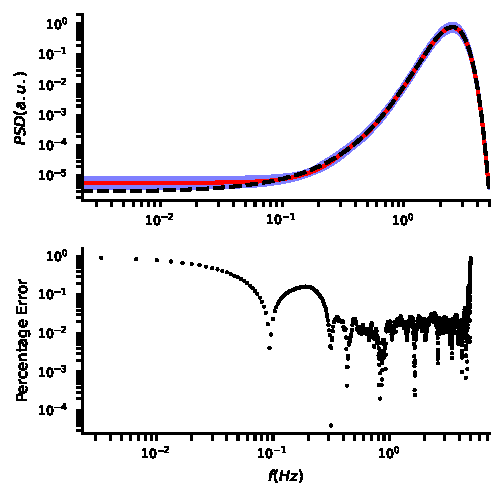
\includegraphics[width = \linewidth]{Images/optimisers_comparison/normal/FPE_spectrum_estim.pdf}
	\caption{Average spectrum for $\mathcal{L}_{\rm FPE}(m)$ with 90\% confidence regions (top) and percentage error (bottom). The average is computed with $1000$ realization of a $3000$ points long time series.}
	\label{fig:FPEmean}
\end{figure}
\begin{figure}[t]
	\centering
	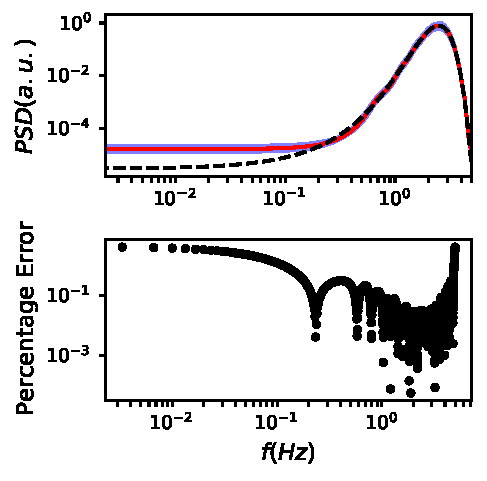
\includegraphics[width = \linewidth]{Images/optimisers_comparison/normal/OBD_spectrum_estim.pdf}
	\caption{Average spectrum for $\mathcal{L}_{\rm OBD}(m)$ loss function with 90\% confidence regions (top) and percentage error (bottom). The average is computed with $1000$ realization of a $3000$ points long time series.}
	\label{fig:OBDmean}
\end{figure}

\begin{figure}[t]
	\centering
	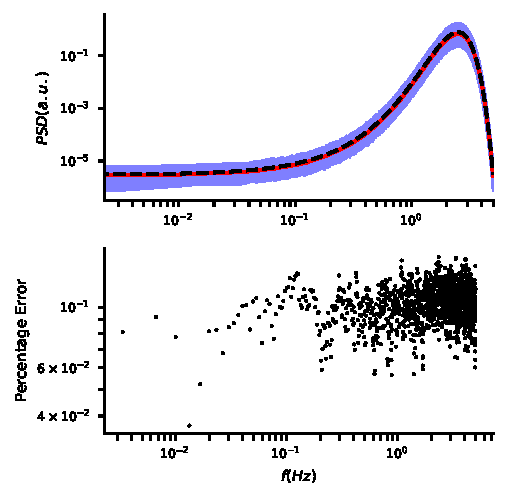
\includegraphics[width = \linewidth]{Images/optimisers_comparison/normal/CAT_spectrum_estim.pdf}
	\caption{Average spectrum for $\mathcal{L}_{\rm CAT}(m)$ loss function with 90\% confidence regions (top) and percentage error (bottom). The average is computed with $1000$ realization of a $3000$ points long time series.}
	\label{fig:CATmean}
\end{figure} 

\begin{figure}
	\centering
	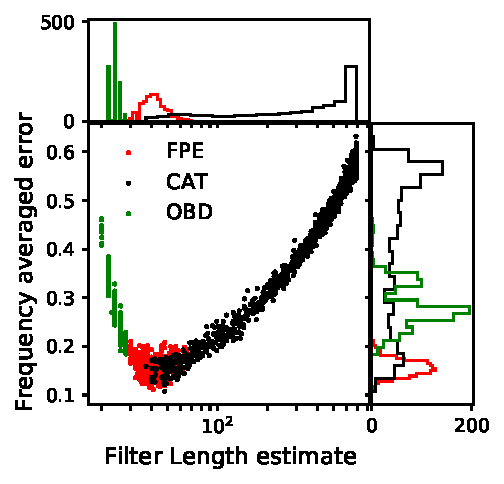
\includegraphics[width = \linewidth]{Images/optimisers_comparison/normal/error_length_contour.pdf}
	\caption{Relative error $r$ (as in eq.~(\ref{eq:freq_error})) vs the length $m$ of autoregressive process, for each of the $1000$ independent realizations of the synthetic time series with gaussian PSD given in Fig.~\ref{fig:autocorr}. Different colours refers to different choices for the loss function: in red $\mathcal{L}_{\rm FPE}(m)$, in green $\mathcal{L}_{\rm OBD}(m)$ and in black $\mathcal{L}_{\rm CAT}(m)$. The top and right histograms show the marginal distributions.}
	\label{fig:optcomparison}
\end{figure}

\paragraph{Final Prediction Error (FPE)}
The results of our investigation on the performance of FPE are shown in Fig.~\ref{fig:FPEmean}.
Qualitatively, there is a good agreement between the reconstructed spectrum and the true spectrum; 
however, we note that the reconstruction is not very accurate in the low frequency region. 
Furthermore, the $90\%$ credible region is very small: this means that if we randomly take two of the reconstructed spectra, we expect their differences to be statistically small. These facts are evidence for FPE to be a reliable loss function.

By looking at therRed series in Fig.~\ref{fig:optcomparison}, we note that the autoregressive orders obtained with FPE are clustered in a very small region. This is a desirable property: FPE, in fact, provides a stable estimation of the autoregressive order, which does not affect much the reconstruction error.
We conclude that the FPE shows good quality reconstruction for the spectrum and very desirable stability properties, its estimate for filter's length $m$ is clustered in a region where there is no dependence of error from $m$. 
\paragraph{Optimum Bayes Decision Rule (OBD)}
The second loss function in consideration is OBD. As for the FPE loss function, the results in Fig.~\ref{fig:OBDmean} show a 
good agreement between the average over the reconstructions and the true spectrum.
Qualitatively the same behaviour of FPE is observed: a good quality reconstruction at the intermediate and high frequencies with a low $90\%$ confidence level; and a worse performance at low frequencies.
However, when looking at the error, the disagreement of this method is found to be larger than the one obtained with FPE: in the worst case, the error can be as large as a factor of $2$ when compared with FPE. 

The error as a function of the autoregressive length (green series in Fig.~\ref{fig:optcomparison}) cluster in a small region, indicating the stability of the reconstructed process order $m$. We note that on average, OBD tends to choose smaller values of $m$ with respect to FPE.

\paragraph{Criterion Autoregressive Transfer function (CAT)}
The performance of CAT is shown in Fig.~\ref{fig:CATmean}. At a first glance CAT differs substantially from the other two loss functions considered.
The ensemble-average PSD matches very well the underlying ``true" PSD. This is also true even in the low frequency region, 
where both OBD and FPE had a poor performance.
However, the variance of the reconstructed spectrum is quite large (much larger than for FPE and OBD), and the relative error is quite high, $\sim 10\%$ and it is approximately constant over all the frequencies.

The reason for this behaviour becomes clear from Fig.~\ref{fig:optcomparison} (black series). CAT does not converge 
to any specific value for the order of the autoregressive process.
In turn, the estimates for the order span a large range of values, hence the large variance observed.
Fig.~\ref{fig:optcomparison} also shows a strong dependence of the error on the estimated length of the filter. The good quality of the reconstruction from the average spectrum can be explained as follows: long filters are able to capture features that short filters cannot see, like outliers in different realization of the time-series, but this is also responsible of an increased variance in the estimate, by introducing spurious peaks in the reproduction.

When averaging the different PSD estimates, the noise in each spectrum cancels, as expected for Gaussian noise. 
This implies, in a sense, that each estimate of the spectrum is independent of any other, as suggested by the huge variance in the residuals. This lack of stability is not a good property for the estimation estimation of the PSD from a single realisation of the time-series, however, thanks to the averaging out of the errors, this estimator seems optimal in the case of repeatable experiments and ensemble-averages.

\paragraph{Final remarks on the choice of the loss function}

In our analysis, the FPE and OBD loss functions are found to behave similarly while CAT shows fairly different properties.
CAT provides an accurate average spectrum over all the frequencies at the price of a large variance; in turn OBD and FPE 
provide a poorer average in the low frequency tails, however they also display a  smaller variance, with FPE showing the lowest.

The poor low-frequency reconstruction from OBD and FPE might be due to the fact that very small values require longer filters. 
In fact, when we consider the average for all the spectra we note that short filters yield larger the error in the tails. OBD, which select the shortest filters, can provide an error as large as $300 \%$ at the extrema, as compared with $85\%$ error of FPE. In turn, CAT is $5\%$ accurate in those regions.

However, we also note, see Fig.~\ref{fig:optcomparison}, that the psD inferred from a single time-series realisation with FPE is still able 
to provide the lowest averaged error over all frequencies, while CAT can reach errors $5$ times larger.
Hence, while CAT is the loss function that minimizes errors in the low-frequency end of the spectrum, 
FPE obtains the best overall accuracy. 

The conclusion is clear: even if in some cases CAT might be more accurate when taking the average over several estimation, FPE guarantees that the single estimation will be more accurate.
As in any common situation we cannot perform such averaging over different realization of the same time series, we must prefer FPE over CAT (let alone OBD, which even though qualitatively similar to FPE has worse performance).
However, if we indeed can measure the PSD by averaging over different time series, using CAT as a loss function is the best choice. In this sense
we retain CAT to provide the best, and most similar in spirit, alternative to the commonly employed WelchPsd estimation method whenever 
ensemble-averages are needed and justified.

%It is evident that tails do not affect CAT  average error and standard deviation at all, so that it's accuracy is approximately constant everywhere in the spectrum. \\ \ 
%Since both FPE and CAT shows pros and cons, at this level, there is no reason to choose between them.\\ 
%Analyzing the resolution of the single reconstruction, figure \ref{fig:optcomparison} clearly shows that FPE minimize overall relative error giving a stable result.\\ 
%CAT instead shows a larger error and do not converge to any specific value. Almost every reproduction obtained with CAT is worst with respect to those obtained with FPE, but their mean is more precise. \\ 
%It's instability is probably the cause for this behaviour. Since it does not show a strong convergence to some order with respect to others, very different lengths are selected.
%Longer lengths are able to capture a lot of details but are more likely to introduce noise. In other words, long filters reduce bias but increment the variance of the result. 
%Taking the average, for central limit theorem the error decreases as $\sim \frac{1}{\sqrt{N}}$. In this way we compensate noise and obtain a spectrum with small bias and small fluctuations.
%Considering the average, CAT reconstruct precisely and with good accuracy every part of the spectrum, even if in "regular" parts best accuracy is reached from FPE. For a single reproduction, CAT is very noisy and unstable, while FPE performs the better. \ref{fig:optcomparison}
%definitely shows that FPE gives the best results: it is a stable method that choose filters in the clustered area associated with minimum error, while both OBD and CAT result lies outside this area and show bigger errors. Two other interesting plots that stress this fact are reported in figure \ref{fig:ordersCompairson} and \ref{fig:residualsComparison}
%where the histograms for the errors and for order's estimate are reported. These graphs provide stronger evidence for our previous statements. As already noticed, FPE is very stable and provide the smallest 'overall relative error'. \\
%CAT histogram shows a very interesting behaviour. The histogram for the order show two different peaks,  a small one associated to 'short filters', and a second high peak at $m = M$. This means that CAT is most likely to not converge at all at some value for the regression order, and it is more likely selects a length that is comparable with the largest available.  If short filters are selected, the overall percentage error will be low, respectively represented by the first peak in the distribution of the errors, while if long filters are selected, the error is maximized. 



\subsection{Choice of the loss function: LIGO Spectrum} \label{sec:LIGO_validation}
We continue our characterisation of the various loss functions considered in this work, by investigating the 
reconstruction of a specific, known, power spectrum: that is the Advanced LIGO design sensitivity theoretical spectral curve\wdp{add ref}.
For this analysis, we generate $500$ time series of $40960$ points each, sampled with a sampling rate of $\SI{2048}{Hz}$, hence we fix the duration
of the time-series to $\SI{20}{s}$. The chosen length is convenient to capture fairly accurately the low-frequency features of the LIGO PSD.

\begin{figure}
    \centering
     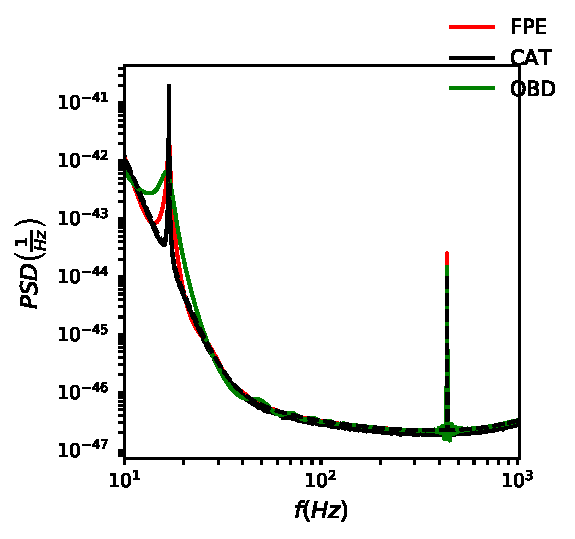
\includegraphics[width = \linewidth]{Images/optimisers_comparison/ligo/compare_estimates.pdf}
      \caption{Average spectrum for the three different loss function as compared with the ``true" PSD. The average is computed with $500$ realization of a $40960$ points long time series.}
       \label{fig:ligospectrum}
\end{figure}
Our findings are summarised in Figs.~\ref{fig:ligospectrum} and ~\ref{fig:LigoOrderError}. The former shows the original spectrum (dashed line)
and the ensemble-averaged reconstructed PSD adopting the FPE (green line), OBD(red line) and CAT(black line). In all cases, the spectrum is well reconstructed, but with a fairly distinct behaviour at low frequency, where CAT -- as in the Gaussian case -- better captures and resolves the distinct 
spectral feature at $\sim 17$ Hz, see also the left panel in Fig.~\ref{fig:ligoPeaks}, as well as the high frequency line at $438$Hz, right panel in Fig.~\ref{fig:ligoPeaks}. 
Fig.~\ref{fig:LigoOrderError} shows the distribution of recovered AR orders $m$ against the relative frequency-averaged error. The behaviour
of the three loss functions is very similar to what found in the Gaussian PSD case: ODB infers the smallest orders and gives average errors around $20$\%, FPE consistently estimates orders of a few hundreds and shows the smallest errors $\sim 15$ \%while CAT does not show any preference towards any AR order and displays wildly varying errors. Yet again, when the PSD is averaged over multiple realization of the time, CAT is able to capture the spectrum very precisely. In fact, even in presence of very sharp peaks, CAT reconstruction seems to be almost perfectly coincident with each of them (figs.\ref{fig:ligoPeaks}).
Hence, also the study of simulated Advanced LIGO data seems to indicate that whenever and wherever ensemble-averaged PSD are necessary, CAT is the optimal choice of loss function. However, on a single time-series realisation, FPE is the more robust choice.

Let us summarise some key general conclusions:
\begin{itemize}
	\item There are no reasons to prefer OBD over CAT or FPE.
	\item If we have one single realization for the process, we recommend the use of FPE, that would get the best resolution possible. In this situation, CAT would provide spurious and unreliable results, with large error.
	\item In the case of several realizations of the same process, CAT ensemble-average properties provide very precise spectral estimation.\end{itemize}

Therefore, the choice of loss function, at least in between CAT and FPE, depends on the problem one  is attempting to solve.
\begin{figure}[t]
        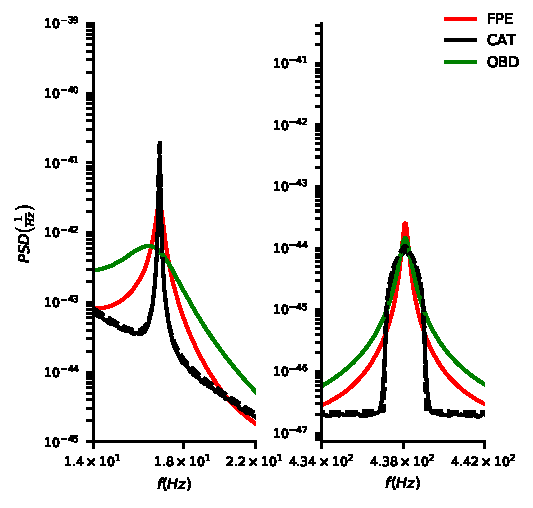
\includegraphics[width = \linewidth]{Images/optimisers_comparison/ligo/compare_estimates_peaks.pdf}
        \caption{Details of peaks of the spectrum and their reconstruction with every optimizer}
        \label{fig:ligoPeaks}
\end{figure}
\begin{figure}
    \centering
    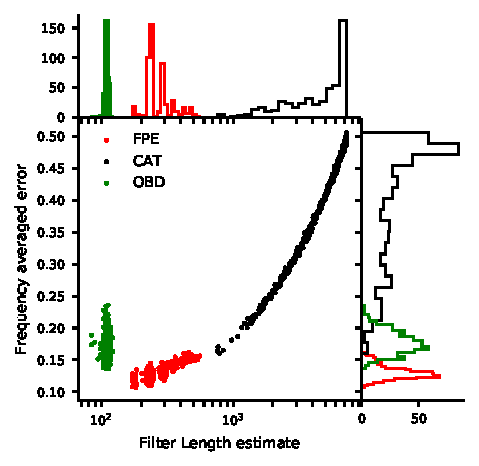
\includegraphics[width = \linewidth]{Images/optimisers_comparison/ligo/error_length_contour.pdf}
    \caption{For each of the $500$ independent realization of the time series, we plot the relative error $r$ (as in eq.~\ref{eq:freq_error}) against the length $m$ of autoregressive process. The time series are randomly drawn with a the analytical LIGO PSD in fig.`\ref{fig:ligospectrum}. Different colors refers to different choices for the loss function. Histograms for the distribution od the individual quantities are also represented.}
    \label{fig:LigoOrderError}
\end{figure}

\subsection{How well the autoregressive order is recovered?}

\begin{figure}
	\centering
	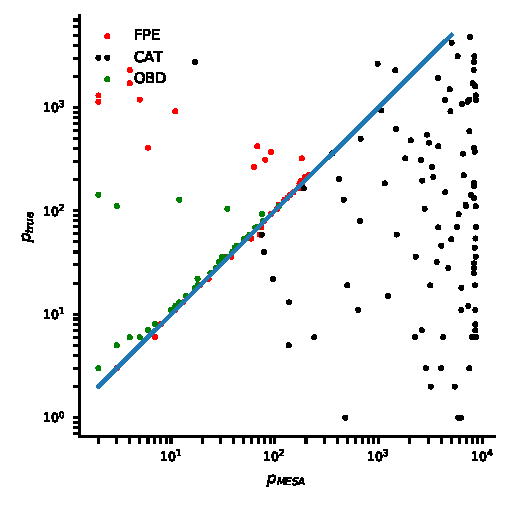
\includegraphics[width = \linewidth]{Images/arp_errors/scatter_deltap_ptrue}
	\caption{Reconstructed value for the autoregressive order plotted against the true value of the autoregressive order.
	The reconstructed autoregressive orders are computed from a time series randomly drawn with an $AR(p)$ model, with the three different loss functions under investigation.
	}
	\label{fig:p_vs_ptrue}
\end{figure}

We now address the issue of how well the autoregressive order (i.e. the number of $a_k$ coefficients employed) is estimated with each loss function.
In doing so, we generate $100$ autoregressive processes $AR(p)$ with a random value of $p$, drawn such that $log(p)~\mathcal{U}_{[log(2), log(5000)]}$.
Each coefficient $a_k$ is assigned according to a Dirichlet distribution $\mathrm{Dir}([1,\hdots, 1])$. The sign of $a_k$ is assigned randomly according to a binomial distribution.
We report the result of this investigation in fig.~\ref{fig:p_vs_ptrue}

Observations below!!!!

\section{Comparison with Welch method}

It is really interesting to have a qualitative comparison between the performance of the MESA and of the standard Welch algorithm.
We perform such comparison on the spectrum of LIGO (even though similar conclusions can be drawn from any other PSD).

We perform two sets of experiments.
In the first one (see fig.~), we simulate data from an analytical PSD and we make the comparison with them: this is to ensure the we have a baseline PSD to compare the data with.
In a second experiment (see fig.~), we employ the data released to the public byt the LIGO/Virgo collaboration.
In each experiment, we vary the length of the data used for the estimation: this is also useful to assess how the computation depends on the data available. We set the total observation time $T = 1, 5, 10, 100, 1000 \SI{}{s}$
For the MESA algorithm, we employ FPE optimizer. For the Welch algorithm, we employ a Tukey window, an overlap fraction of $0.5$ for the segments and a length of segments $L = 512, 1024, 2048, 8192, 32768$ datapoints.
In all cases, the sampling rate is set to $\SI{4096}{Hz}$.

First of all, we note that using a longer time series results in a more stable estimation of the PSD, especially in the low frequency sector. This is somehow obvious: more data provide more information available for spectral estimation. This fact is more important at lower frequencies, where the natural time length is large.

Turning to the comparison between MESA and Welch's method, we find that the PSD estimation provided by the Welch's method is more noisy (i.e. has a large number of spurious peaks) rather than PSD provided by MESA. The different behavior is more manifest in the low frequency sector.
The result does not change much by changing the hyperparameters required for Welch algorithm.
\sschmidt{Other observations??}


\begin{figure}
	\label{fig:mem_welch_realdata}
	\caption{Make here a comparison between Welch - True data}
	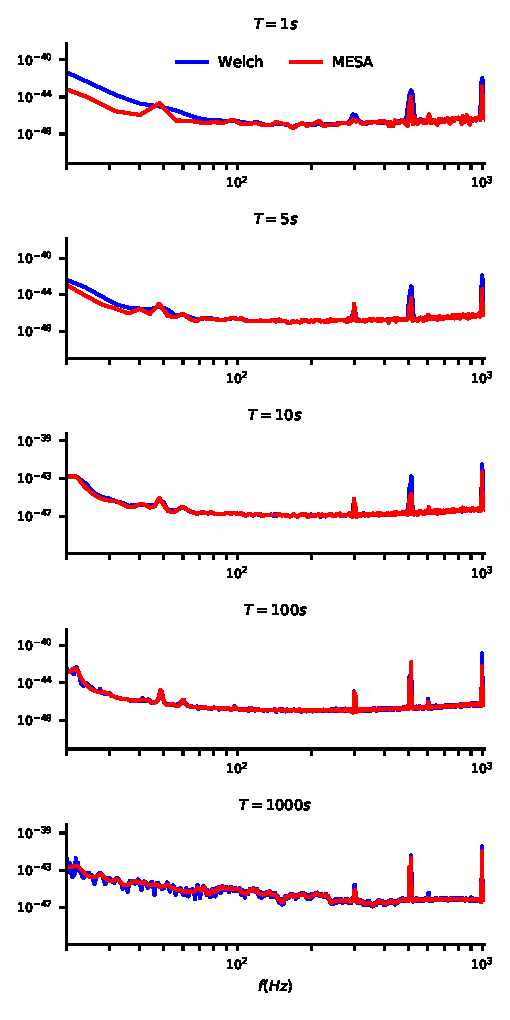
\includegraphics{Images/comparison_LVC_data/comparison_LVC_data_overall_fake_False.pdf}
\end{figure}
\begin{figure}
	\label{fig:mem_welch_fakedata}
	\caption{Make here a comparison between Welch - Fake data}
	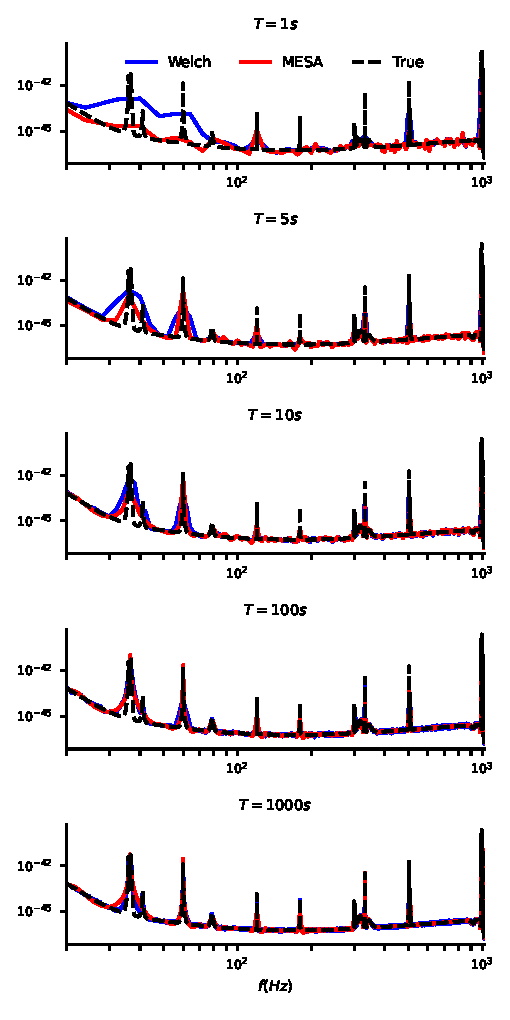
\includegraphics{Images/comparison_LVC_data/comparison_LVC_data_overall_fake_True.pdf}
\end{figure}

\sschmidt{Mettiamo da qualche parte una descrizione dettagliata del codice? No: solo rimandiamo al codice nell'intro}

\section{Forecast analysis}
\section{Final remarks and future prospects}

\appendix
\section{MESA solution} \label{sec:MESA_solution}
\subsection{MESA solution}
To derive the expression for the MAXENT spectral estimator the approach proposed by Burg \cite{burg1975maximum} will be followed. The constraints \ref{eq:MaxConstraint} are not implemented via the standard Lagrange Multipliers approach while the entropy gain \ref{eq:EntropyGain} will be re-written by explicitly writing $S(f)$ as the Fourier Transform of the sample autocorrelation function: 
\begin{equation}
    S(f) = \frac{1}{2 Ny}\sum_{n = -\infty}^{\infty} \bar r_n e^{- \imath 2 \pi n \Delta t},
\end{equation}
and becomes
\begin{equation}
    \Delta H = \int_{-Ny}^{Ny}  
    \log\left(\frac{1}{2 Ny}\sum_{n = -\infty}^{\infty} \bar r(n\Delta t) e^{-\imath 2 \pi f n \Delta t} 
    \right) df.
\end{equation}
Deriving with respect to the autocorrelation function $r_s$
\begin{equation}
      \frac{\delta H}{\delta \bar r_s} = \frac{1}{2Ny}\int_{-Ny}^{Ny} S(f)^{-1}e^{-\imath 2 \pi f s \Delta t } df = \lambda_s. 
\end{equation} 
its easily shown that $S(f)^{-1}$ can be written as a Fourier Expansion in terms of some $\lambda$s coefficients. The determination of the values for the $\lambda$s uniquely solve the problem of power-spectral density estimation. Some properties for the coefficients can be worked out easily. First, since $S(f)$ is positive definite the $\lambda$s coefficient show the property 
\begin{equation}
\nonumber 
\lambda_s = \lambda_{-s}^*. 
\end{equation}
The second property is obtained considering that the autocorrelation function can only be computed for a finite time interval $n \in [-N, N]$, the requirement for our estimate to be independent from the unkown values of the autocorrelation function can be implemented as:  
\begin{equation}\nonumber 
    \frac{\delta H}{\delta \bar r_s} = 0 \text{ for } \vert s \vert > N,
\end{equation}
that means 
\begin{equation}
\nonumber 
\lambda_s = 0 \text{ for } \vert s \vert > N. 
\end{equation}
From the previous equations is easily seen that $S(f)$ can be expressed via a Fourier Series 
\begin{equation}\label{eq:PSDconstraint}
    S(f)^{-1} = \sum_{s = -N}^N \lambda_s e^{-\imath 2 \pi f s \Delta t}.
\end{equation}
Defining $z = e^{-\imath 2 \pi f \Delta t}$ the previous Fourier expansion becomes a Laurent Polynomial in $z$: 
\begin{equation}
    \label{eq:zExp}
    S(f)^{-1} = \lambda_0 + \sum_{s = 1}^N \lambda_s z^s + \sum_{s = 1}^N \lambda^*_s z^{-s}.
\end{equation}
It is easy to show that if $z_0$ is a root for the polynomial $(z_0^*)^{-1}$ is also a root: for every root laying outside the unit circle there will be another root inside of it and vice-versa. These properties allow us to rewrite the Fourier expansion (\ref{eq:zExp}) as \cite{1975STIN...7714318B}:
\begin{equation}\label{eq:MESApsd_appendix}
    S(f) = \frac{P_N \Delta t}{\left(\sum_{s=0}^N a_s z^z\right)\left(\sum_{s = 0}^N a^*_s z^{-s}\right)}
\end{equation}
with $a_0 = 1$ and $\Delta t$ the uniform sampling interval for the time series. The vector obtained as $(1, a_1, \dots, a_N)$ is known as the prediction error filter. The power spectral density $S(f)$ is uniquely determined if both the prediction error filter and $P_N$ coefficients are computed. \\
To compute the $a_i$-s it is convenient to rewerite the equation 
(\ref{eq:MaxConstraint}) in terms of the Laurent Polynomial and then integrating over $z$. In this way the equation becomes:
\begin{equation}
   \frac{P_N}{2 \pi \imath} \oint _{\mathbb S^1}\frac{z^{-s - 1}}{\sum_{n = 0}^N a_n z^n \sum_{n = 0}^N a^*_n z^{-n}}dz = \bar r_s. 
\end{equation}
Substituting $s \to s - r$, multiplying by $a^*_s$ and summing over $s$ the previous equation becomes 
\begin{equation}
    \sum_{s = 0}^N a_s \bar r_{s - r} = \frac{P_N}{2 \pi \imath}\oint \frac{z^{r -1}}{\sum_{s = 0}^N a_s z^s}dz.\label{eq:ErFilter}
\end{equation}
From now on only wide-sense stationary processes will be considered: for such a process all poles lay outside the unit circle so that the previous integral can be easily computed obtaining the following, well known, equations: 
\begin{align}\label{eq:errorFilter1}
    \sum_{s = 0}^N a_s \bar r_{r - s} &= P_N \quad \text{ if } r = 0 \\ \label{eq:errorFilter2}
    \sum_{s = 0}^N a_s \bar r_{r - s} & = 0 \qquad \text{ if } r \neq 0.
\end{align}
The solution of the previous equations fully determine the functional form of the power spectral density estimator \ref{eq:MESApsd_appendix}, and the method for solving such equations is the Levinson-Durbin recursion \cite{doi:10.1002/sapm1946251261}. The recursion can be easily schemitized as follows: 
After defining the quantities  
\begin{align}
\Delta_N &= \sum_{n = 0}^{N}R(N - n + 1)a_n \\ 
c_N &= - \frac{\Delta_N}{P_N},
\end{align} the Levinson recursion is: 
\begin{equation} \label{eq:Levinson1}
P_N = P_{N -1}\left(1 - \vert c_{N - 1} \vert ^2\right)
\end{equation}
and 
\begin{equation} \label{eq:Levinson2}
\begin{pmatrix}
1 \\ a_1 \\ \vdots \\ a_{N - 1} \\ a_N
\end{pmatrix}
= 
\begin{pmatrix}
1 \\ b_1 \\ \vdots \\ b_{N -1} \\ 0
\end{pmatrix}
+ c_{N-1}
\begin{pmatrix}
0 \\ b_{N -1}^* \\ \vdots \\ b^*_1 \\ 1
\end{pmatrix}. 
\end{equation}
with $b$ the forward prediction error coefficients at order $N-1$. 
The 0'th order element can be easily initialized reminding that $a_0 = 1$ whatever the order the other coefficients. $P_0$ can be determined from \ref{eq:errorFilter1} and its value is: 
\begin{equation}
P_0 = R(0),
\end{equation}
 while $\Delta_0$ and $c_0$ are uniquely determined from their definitions and are
\begin{equation}
\Delta_0 = R(1); \quad c_0 = -\frac{R(1)}{R(0)}. 
\end{equation}
These expressions allow us to compute $\vec a$ and $P_N$ to whatever order by simply iterating \ref{eq:Levinson1} and \ref{eq:Levinson2}. Substituing them in equation \ref{eq:MESApsd_appendix} the problem of the estimation for the power spectral density via maximum entropy principle is solved. While Burg's method for spectral analysis is solved via Levinson recursion, another faster recursion \cite{Vos} is implemented in memspectrum package.


	\bibliography{Bibliography.bib}
	\bibliographystyle{ieeetr}

\end{document}

